\section{Design Overview}
\label{sec:design}

Delivering messages, important and casual, to mobile users and
endpoints that are interested in them is the overarching premise of
this work. Our vision for realizing an end-to-end mobile message
delivery service design principles revolve around four central
goals:

\begin{itemize}
\item Relevant content

The service should provide mechanisms to target groups of endpoints
which have explicit or implied interest in messages. A message may be
important because an end user specifically asked for the content based
on its attributes (nearby gas prices). Alternatively, a message may be
deemed relevant for the endpoint because it is related to an emergent
event (vehicle accident ahead).

\item Robust, low overhead, low latency communication

Message intent drives content delivery requirements.  For example,
different types of emergency service messages have been identified for
VANETs, each having distinct latency
requirements~\cite{camp2005vehicle}. The service should strive to
minimize latency to provide on-time delivery with headroom for outlier
delays. Messages should be categoriezed according to their relative
importance and processed accordingly (e.g., emergency info before
consumer content).

\item Flexible deployment

Adoption of the service is bolstered by adaptability to different
mobile networking environments.  Such accomodation allows for
deployment into LTE networks with different geographic EPC service
placements and degrees of maleability.  The service should allow for
centralized metropolitan area integration (CloudRAN) and distributed
edge deployment (peer-to-peer eNodeB).

\item Reuse of effective technologies

It is our contention that an end-to-end service should not supplant
existing mechanisms useful for achieveing its composition.  Indeed, it
is counterproductive to introduce new service components that induce
unnecessary changes and capital investments. The messaging service
should strive to work alongside existing mobile network protocols and
services.  Only where existing mechanisms do not provide key
functionality or do not give adequate service levels should changes be
introduced.  Such changes should be as minimal and transparent as
possible to foster compatibility and ease of adoption. On the other
hand, considering less constrained future mobile network
architectures~\cite{5gvision,venkataramani2014mobility} is also
important.

\end{itemize}

We next describe the components of the \name~messaging system, along
with how they fit into the 3GPP 4G mobile networking architecture.

%%% ARCHITECTURE FIGURE
\begin{figure*}[ht]
  \centering
  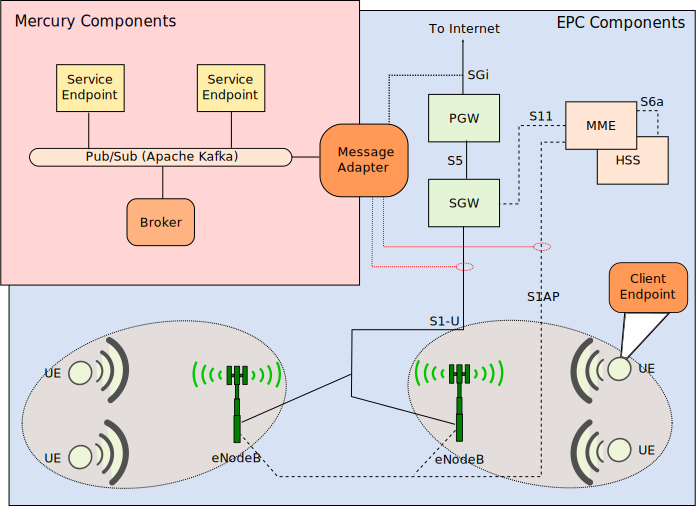
\includegraphics[width=0.8\textwidth]{figs/mercury-arch.png}
  \caption{\name~architecture diagram (in 4G mobile network context)}
  \label{fig:arch}
\end{figure*}

\subsection{\name~Components}

\name~is comprised of four essential components: message broker,
publish/subscribe system, message adapter, and endpoints.  These
components are visible in the architecture diagram in
figure~\ref{fig:arch}. This diagram shows the \name~components
in the context of a 4G mobile network (the latter will be described
after \name~is covered).

\subsubsection{Message Broker}

\name's message broker is the brain center of the messaging
system. It processes all incoming messages and sends these to relevant
endpoints (via \pubsub). The broker calculates Areas of Interest (see
section~\ref{sec:aoi}) for certain message types (e.g., emergency
notifications).  Data analysis (aggregated decisions, client
statistics, etc.) occur at the broker. It does not concern itself with
how to get the messages to the target endpoint(s); that job falls to
the \name~message adapter.

\subsubsection{Publish/Subscribe System}

\name~needs a pubsub system that can serve a high number of events
with low latency. This is because of the environment in which it
operates.  We have many agents/endpoints at any given point that
interact with the system and for them to effectively respond to a
situation we need to dissipate the messages quickly. The mobility of
the clients creates the potential for intermitent loss of connectivity
with the pubsub system which has to be re-established. Among the options
considered, Apache Kafka had the best combination of low-latency and
message queueing for recovering lost messages.

At a high-level Kafka gives the following guarantees: Messages sent by a 
producer to a particular topic partition will be appended in the order they are
sent. A consumer instance sees records in the order they are stored in the log. 
For a topic with replication factor N, kafka will tolerate up to N-1 server 
failures without losing any records committed to the log.

\subsubsection{Message Adapter}

The \name~message adapter is the conduit through which pubsub
messages flow through to endpoints. The adapter coordinates sessions
with client endpoints. It forwards client reports and other content to
and from the pubsub. It also maintains pubsub topic subscriptions for
the endpoints. The prototype implementation described in this
paper targets the 4G EPC, but it is possible to target other mobile
networking architectures with different adapters.

\subsubsection{Endpoints}

\name~endpoints are the producers and consumers of most content in
the messaging system. Client Endpoints run as applications on
ITS-equipped vehicles.  They report in with telemetry, such as their
current position and speed.  Client endpoints also subscribe to
particular consumer messages identified by specified attributes.

Service Endpoints may also be centralized services that connect to the
pubsub, running at the same location as the Broker, and using the
Broker's services. Examples include emergency notification processors,
and consumer information aggregators (gas prices).

\subsection{\name~Messages}

Messages are the principle and only communication mechanism in
\name. There are two high-level flavors: control and
content. Control messages include session handling (between broker and
endpoints), broker to message adapter communication, and subscription
management (endpoint to pubsub/broker).  Content messages are those
relevant to applications running on endpoints, such as emergency
alerts and consumer information (e.g. gas prices).  Periodic session
maintenance messages are sent between the mobile endpoints and the
\name~Adapter to update status (location) and track liveness.

%The broker likewise sends periodic
%heartbeat messages toward all endpoints. These messages ensure clients
%and broker stay in sync. Session handling also includes establishment
%and teardown message exchange.  

Content messages use structured 
message attributes to signal category information. This allows content
producer and consumer endpoints to steer messages to one another based
on interests. Most messages (including client reports) flow through
the pubsub system to the broker. This allows the Broker to perform
data aggregation and analysis (triggers based on thresholds, for
example).

Message destination addressing in \name~includes endpoint, content,
and area of interest targetting. Endpoint addresses are primarily used
for session setup and teardown. Content-specific addressing makes use
of subscription attributes to deliver messages. AOI addresses are
unique to the mobile environment. AOI bounds are computed by the
broker. These bounds form the destination address. Message adapters
check bounds to determine if their downstream area coverage is
relevant before passing along, and endpoints check their position
relative to the bounds.  In this way, \name~allows messages to be
``area multicasted.''  As we discuss in
section~\ref{sec:design-details}, our prototype restricts itself to
simple bounding models (radius). Complex spatial reasoning for
improving relevancy is left for future work.

%%%%%%%%%%%%%%%%%%%%%%%%%%%%%%%%%%%%%%%%%%%%%%%%%%%%%%%%%%%%%%%%%%%%%%%%%%%%%%
%
% Old text on the pubsub that was too detailed.
%

\comment{
Apache ActiveMQ\cite{activemq} is one of the oldest player
in this space. Though, ActiveMQ messaging is reliable it's performance forms a
bottle neck to our system. RabbitMQ\cite{rabbitmq} is a widely used message 
broker with huge documentation. It is written in Erlang which is suitable for 
distributed applications, as concurrency and availability are well-supported.
However, It relies on synchronous delivery of messages that decreases the numbe
r of events being served. ZeroMQ\cite{zeromq} is another class of pub-sub 
systems that is designed for high throughput/low latency scenarios. 
Yet, most of the features will have to be implemented by ourselves combining 
various pieces of the framework. Redis is an in-memory data structure store, 
used as database, cache and message broker. Redis needs to have as much memory 
as there are messages in flight making it more attractive for short living 
messages and where we don't have a huge consumer capacity so as to not run out 
of memory.

Finally, we have crossed upon Apache Kafka. It is a pub-sub system written by 
linkedin and is under open source license of Apache. Apache Kafka addresses many
of these problems mentioned above. It is very fast and the number of 
messages/events it serves are way more than any traditional pub-sub system. 
It can handle bursts without any out of memory issues. Also, It guarantees 
event ordering. This helps us in going back in time and reading a message that
has been previously published to Kafka. We can seek old messages by remembering 
the offset. In a mobile environment this is very useful as we could see frequent
disconnections. All these attractive features made us choose Kafka as the 
pub-sub system for mercury. Below, we write briefly about different concepts of 
Kafka.

%
% Some text cut/paste from here and put into the implementation section.
%

Kafka has a beautiful concept called Consumer Groups. Consumer Groups can be 
defined as set of consumers subscribed to single topic and each consumer is 
assigned a different partition. We can have multiple consumer groups listening 
to same topic or different. This concept of forming Consumer Groups helps kafka
serve advantages of both message queue and a message-broker. Message Queues and 
message -broker systems have both strengths and a weaknesses. The strength of
queuing is that it allows us to divide the processing of data over multiple
consumer instances, which lets you scale your processing. But, queues can't be
multi-subscribed—once one process reads the data it's gone. Publish-subscribe 
allows you broadcast data to multiple processes, but has no way of scaling 
processing since every message goes to every subscriber. The consumer group 
concept in Kafka generalizes these two concepts. As with a queue the consumer 
group allows you to divide up processing over a collection of processes 
(the members of the consumer group). As with publish-subscribe,
Kafka allows you to broadcast messages to multiple consumer groups. The 
advantage of this model is that every topic has both these properties—it can 
scale processing and is also multi-subscriber—there is no need to choose one or
the other. This is something which we can take advantage of to scale Message 
Broker horizontally.


Kafka has four main APIs: The Producer API allows an application to publish a 
stream records to one or more Kafka topics. Producers publish data to the topics
of their choice. 
The Consumer API allows an application to subscribe to one
or more topics and process the stream of records produced to them. 
The Streams API allows an application to act as a stream processor, consuming an
input stream from one or more topics and producing an output stream to one or 
more output.
The Connector API allows building and running reusable producers or consumers 
that connect Kafka topics to existing applications or data systems. 
We use Producer API and Consumer API extensively in our implementation.
}
